% !TeX root = ../main.tex
% Add the above to each chapter to make compiling the PDF easier in some editors.

\chapter{Lagrange Multipliers and Duality}\label{cha:lagrange_multipliers_duality}

\section{Separating Hyperplanes}

\begin{defn}[Hyperplane] A \emph{hyperplane}\index{hyperplane} of dimension $n$ is the subset, \begin{align}
    \sH(\vn,\mu) \defeq \{\vx \in \R^n \mid \trans{\vn}\vx = \mu\},
\end{align} for some \emph{normal}\index{normal vector} $\vn \in \R^n \setminus \{\vZero\}$ and \emph{threshold} $\mu \in \R$.
\end{defn}

Every hyperplane divides $\R^n$ into two half-spaces $\{\vx \mid \trans{\vn}\vx \leq \mu\}$ and $\{\vx \mid \trans{\vn}\vx \geq \mu\}$. It separates two sets, if they lie in different half-spaces.

\begin{defn}[Separating hyperplane] We say a hyperplane $\sH$ \emph{separates}\index{separating hyperplane} two sets $\sA, \sB$ iff \begin{align}\begin{split}
    \forall a \in \sA: \trans{\vn}\va &\leq \mu \quad\text{and} \\
    \forall b \in \sB: \trans{\vn}\vb &\geq \mu.
\end{split}\end{align} If the inequalities are strict, we say that $\sH$ \emph{strictly} separates $\sA$ and $\sB$.
\end{defn}

If $\sA, \sB$ are non-convex, we are not guaranteed that a separating hyperplane exists (e.g., a point cannot be separated from a ring around it). However, if we assume that $\mA$ and $\mB$ are convex, a separating hyperplane always exists.

\begin{fct}[Separating hyperplane theorem]\index{Separating hyperplane theoerm} Given two disjoint and non-empty convex subsets $\sA, \sB \subseteq \R^n$, there exists a separating hyperplane.
\end{fct}

However, it is not true that there always exists a strictly separating hyperplane. Consider $\sA \defeq \{(x,y) \mid x \leq 0\}$ and $\sB \defeq \{(x,y) \mid x > 0 \text{ and } y \geq \frac{1}{x}\}$. Clearly they are disjoint and convex; however, the only separating hyperplane is $\sH = \{(x,y) \mid x = 0\}$, which intersects $\sA$.
\begin{marginfigure}
TBD
% \centering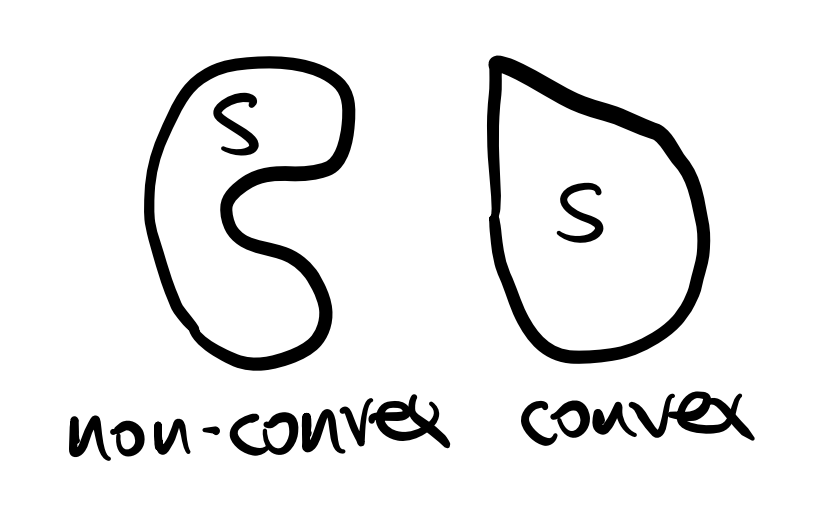
\includegraphics[width=4cm]{notes/figures/convex_set.png}
\caption{Example where no strictly separating hyperplane exists.}
\end{marginfigure}

When we also assume that $\sA$ and $\sB$ are closed and bounded, a strictly separating hyperplane always exists.

\begin{thm}[Separating hyperplane theorem; closed, bounded sets] Given two disjoint, closed, bounded, and non-empty convex subsets $\sA, \sB \subseteq \R^n$, there exists a strictly separating hyperplane.

If $\vc \in \sA, \vd \in \sB$ are minimizers of $\min_{\va \in \sA,\ \vb \in \sB} \norm{\va - \vb}_2$, then one such hyperplane is given by, \begin{align}
    \vn \defeq \vd - \vc \quad\text{and}\quad \mu \defeq \frac{1}{2}\parentheses*{\norm{\vd}_2^2 - \norm{\vc}_2^2}.
\end{align}
\begin{marginfigure}
TBD
% \centering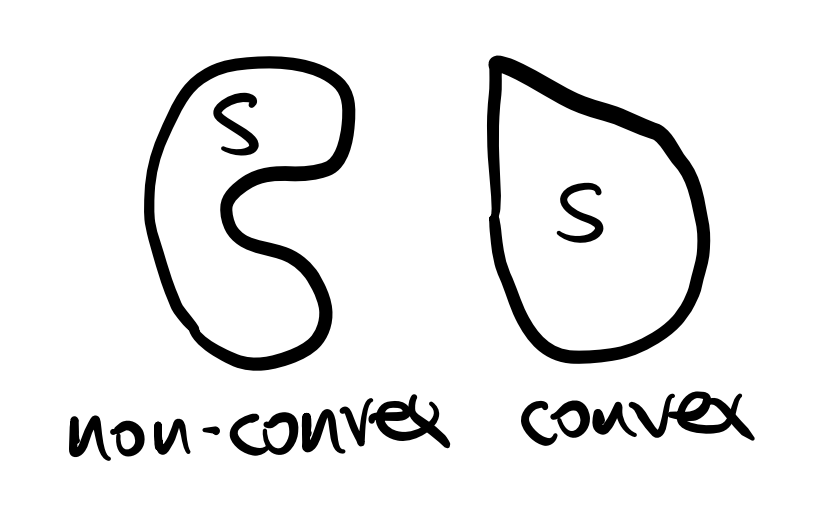
\includegraphics[width=4cm]{notes/figures/convex_set.png}
\caption{Illustration of strictly separating hyperplane.}
\end{marginfigure}
\end{thm}
\begin{proof}
We want to show that $\trans{\vn}\vb > \mu$ for all $\vb \in \sB$. Then, $\trans{\vn}\va < \mu$ for all $\va \in \sA$ follows by symmetry. We have, \begin{align*}
    \trans{\vn}\vd - \mu &= \trans{(\vd - \vc)}\vd - \frac{1}{2}\parentheses*{\norm{\vd}_2^2 - \norm{\vc}_2^2} \\
    &= \norm{\vd}_2^2 - \trans{\vd}\vc - \frac{1}{2}\norm{\vd}_2^2 + \frac{1}{2}\norm{\vc}_2^2 \\
    &= \frac{1}{2}\norm{\vd - \vc}_2^2 > 0. \margintag{using the asusmption that $\sA,\sB$ are disjoint, close, and bounded, their distance is positive}
\end{align*} Suppose for a contradiction that there exists a $\vu \in \sB$ such that $\trans{\vn}\vu - \mu \leq 0$.

Consider the line defined by the distance minimizer $\vd$ and the point on the ``wrong side'' $\vu$, $\vb(\lambda) \defeq \vd + \lambda(\vu - \vd)$. Taking the derivative of the distance between $\vb(\lambda)$ and $\vc$ and evaluating it at $\lambda = 0$ (which is when $\vb(\lambda) = \vd$), we obtain, \begin{align*}
    \left.\odv{}{\lambda}\norm{\vb(\lambda)-\vc}_2^2\right\vert_{\lambda=0} &= \left.2 \trans{(\vd - \lambda\vd + \lambda\vu - \vc)}(\vu-\vd)\right\vert_{\lambda=0} \\
    &= 2 \trans{(\vd - \vc)}(\vu - \vd).
\end{align*} However, \begin{align*}
    \trans{\vn}\vu - \mu = \trans{(\vd - \vc)}(\vu - \vd) + \underbrace{\trans{\vn}\vd - \mu}_{>0} \leq 0,
\end{align*} implies that $\trans{(\vd - \vc)}(\vu - \vd)$, and hence, the gradient are negative, which contradicts the minimality of $\vd$.
\end{proof}

% \section{Fenchel Conjugates}